\subsubsection{User Interface}
% \subsubsection{UML Description}
The UML below describes at high-level the model of the system to be developed. It considers the basic service together with the advanced function 1 and advanced function 2 previously specified. The UML does not include every class that will be necessary to define the complete architecture of the system.\\
CLup more functions than basic service. The manager registers to the application with all necessary information and the manager could activate the advance function or advance function 2 at any time. The user who use mobile could simply download the application on his/her device and use it and user who doesn't have mobile could easily go near the shop and get a ticket from ticket machine.\\
Here we can identify the main aspect of CLup:
\begin{itemize}
    \item The user could request to be in line for a shop and application shows estimated waiting time to him/her.
    \item The user could book a visit for a shop. This booking contains the date and time user wants to go shopping besides, user can add the categories of item he/she has in shopping list. The application could suggest the user free slots and user book them.
    \item The application based the current location of users must notify them and ask them to approach the shop in a suitable time.
    \item The application must notify people when it's their turn to go shopping.
    \item At the entrance time, the QR code generated in the app must be scanned to ensure they come in the right time.
    \item At the checkout, the cashier must scan the QR code of user and the system must add shopping information (like duration of shopping, category of item which user buy) to user history.
\end{itemize}

\begin{figure}[H]
  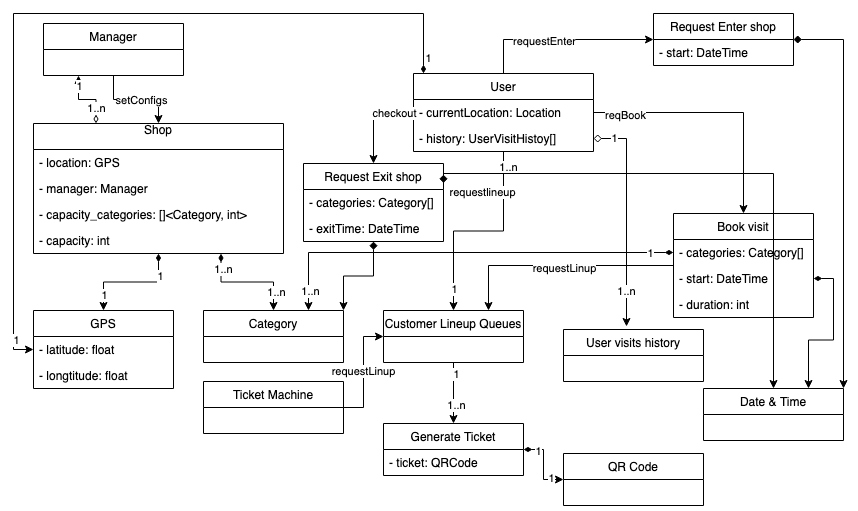
\includegraphics[width=\textwidth,height=\textheight,keepaspectratio]{images/ClassDiagram.png}
  \caption{High level Class Diagram}
  \label{fig:ClassDiagram}
\end{figure}

\subsubsection{State Diagrams}
Now we analyse the some important functions of the application, modelling their behaviours and analyze their behaviour to have the expected functionality. we report these diagrams below. \\

\begin{figure}[H]
  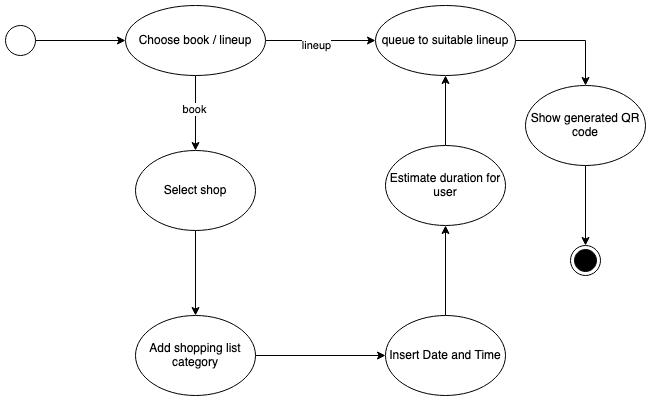
\includegraphics[width=\textwidth,height=\textheight,keepaspectratio]{images/bookLineup.png}
  \caption{User book a visit or insert to lineup queue}
  \label{fig:bookLineup}
\end{figure}

In this (Figure \ref{fig:bookLineup}), we model a user whom has a cell phone and wants to go shopping. As you can see, the user can choose to go to queue or book a visit for a time in future. System could sends him/her list of suggested time and user could choose between them.

\begin{figure}[H]
  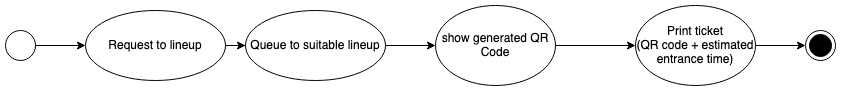
\includegraphics[width=\textwidth,height=\textheight,keepaspectratio]{images/OfflineTicket.png}
  \caption{User get ticket from ticket machine}
  \label{fig:OfflineTicket}
\end{figure}

In this (Figure \ref{fig:OfflineTicket}), we model a user who want to use ticket machine and do not use the app. In this case, user only can add himself/herself to the current line up of the shop.

\begin{figure}[H]
  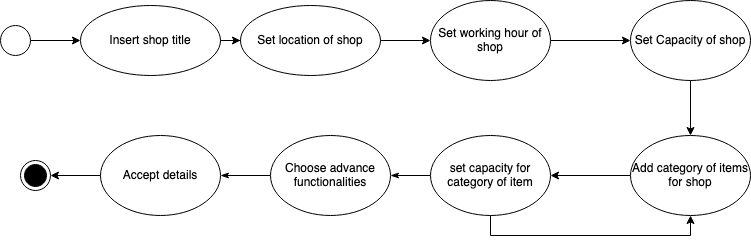
\includegraphics[width=\textwidth,height=\textheight,keepaspectratio]{images/CreateShop.png}
  \caption{Manager create a shop}
  \label{fig:CreateShop}
\end{figure}

In this (Figure \ref{fig:CreateShop}), shows how a manager could create a shop and add necessary information for creating a shop in our system.

\begin{figure}[H]
  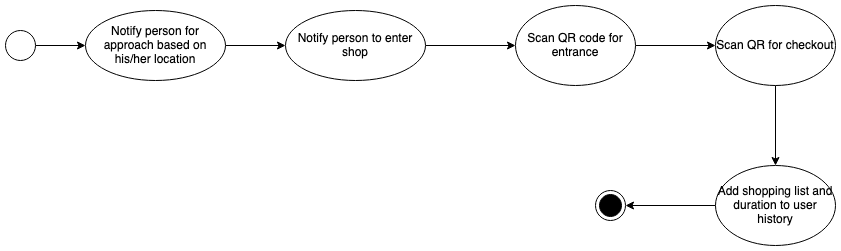
\includegraphics[width=\textwidth,height=\textheight,keepaspectratio]{images/Shopping.png}
  \caption{User shopping}
  \label{fig:shopping}
\end{figure}

In this (Figure \ref{fig:shopping}), we model the behaviour of user from entrance to shop until checkout. In the checkout time, we re-scan the QR code of user to insert data user shopping list and duration to user history. we could use, this information to estimate the behaviour of each user and improve waiting time estimation in our system.
The application that we are using should be able to generate QR codes and will appear in the screen for customers to use. before that, we assume that users already inserted the specific shop they want to go and also choose between two mode of lining up and book a visit for that supermarket later. the app show  estimated time and the number of people before that user so they can save their time and  mange their life better. after all they will scan their QR code and enter the supermarket.
A smartphone and within that, the application, is the suitable thing that answer the needs.
the following mockups give the idea of:
1. The logo of the application looks like;
2. The splash screens;
3. And the 4 first pages of the application;
\begin{figure}[H]
  \centering
  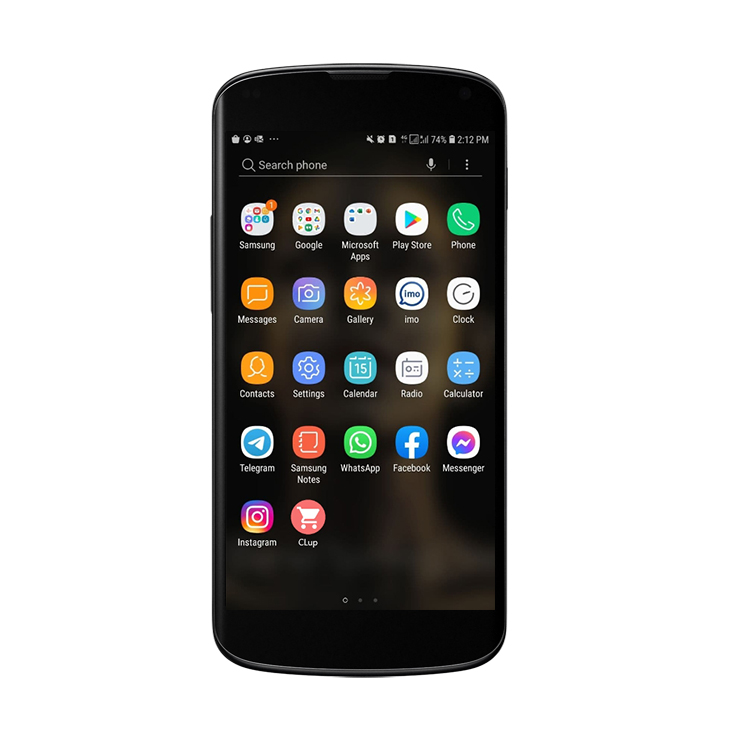
\includegraphics[width=0.7\textwidth,keepaspectratio]{images/1.jpg}
  \caption{Icon Mockup}
\end{figure}
\begin{figure}[H]
  \centering
  \subfloat[Opening page Mockup] {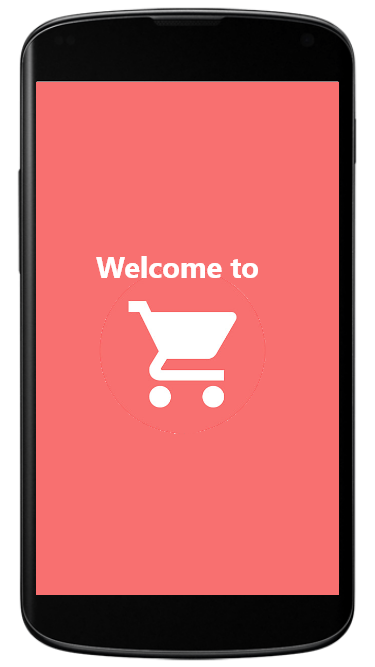
\includegraphics[width=0.4\textwidth,keepaspectratio]{images/2.png}}
  \hfill
  \subfloat[Splash Screen Mockup] {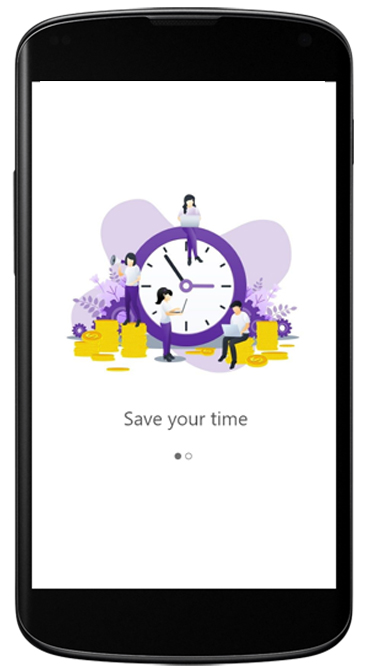
\includegraphics[width=0.4\textwidth,keepaspectratio]{images/3.jpg}}
  \hfill
  \subfloat[Splash Screen page Mockup] {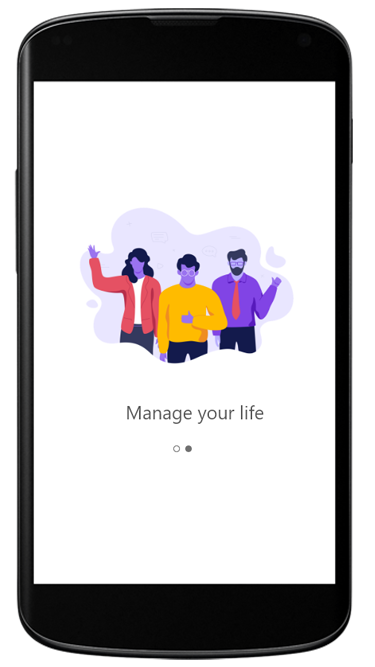
\includegraphics[width=0.4\textwidth,keepaspectratio]{images/4.png}}
  \hfill
  \subfloat[Sign up/log in page Mockup] {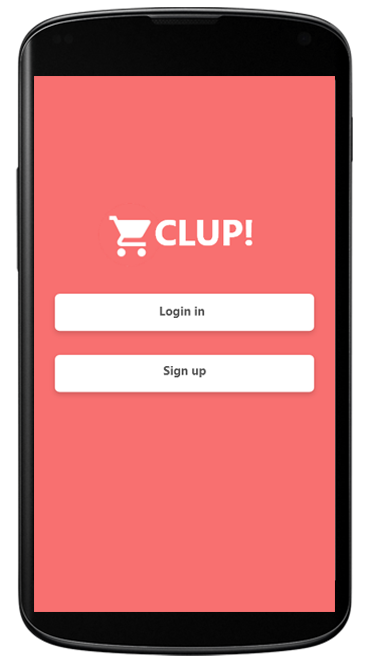
\includegraphics[width=0.4\textwidth,keepaspectratio]{images/5.png}}
  \hfill
  \caption{Mockup}
\end{figure}

\begin{figure}[H]
  \centering
  \subfloat[Log in page Mockup] {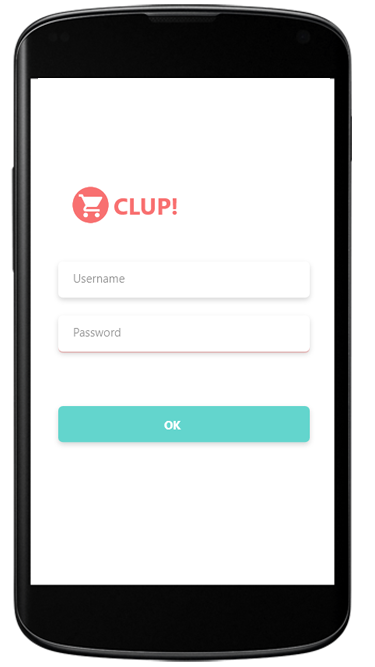
\includegraphics[width=0.4\textwidth,keepaspectratio]{images/6.png}}
  \hfill
  \subfloat[Sign up page Mockup] {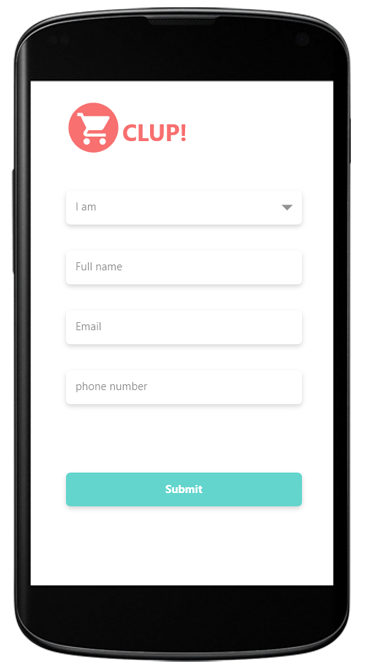
\includegraphics[width=0.4\textwidth,keepaspectratio]{images/7.png}}
  \hfill
  \subfloat[Sign up page II Mockup] {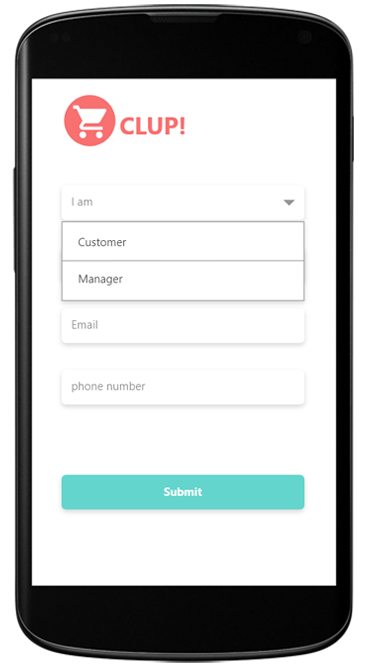
\includegraphics[width=0.4\textwidth,keepaspectratio]{images/8.png}}
  \hfill
  \subfloat[Home page Mockup] {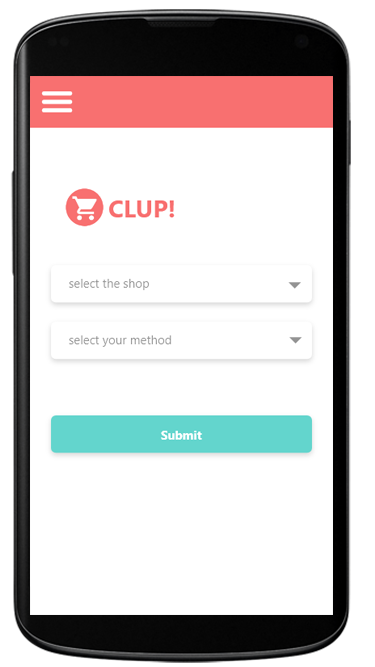
\includegraphics[width=0.4\textwidth,keepaspectratio]{images/9.png}}
  \hfill
  \caption{Mockup}
\end{figure}

\begin{figure}[H]
  \centering
  \subfloat[Home page II Mockup] {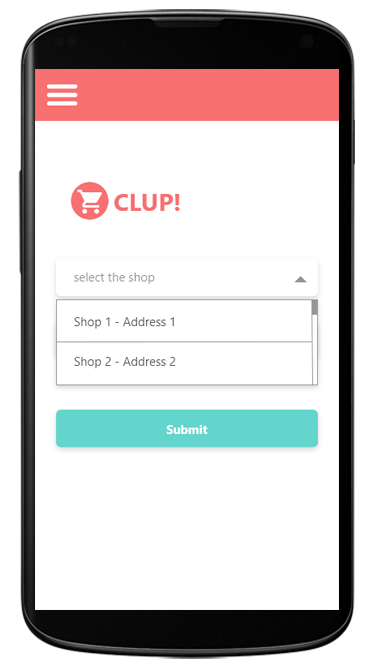
\includegraphics[width=0.4\textwidth,keepaspectratio]{images/10.png}}
  \hfill
  \subfloat[Home page III Mockup] {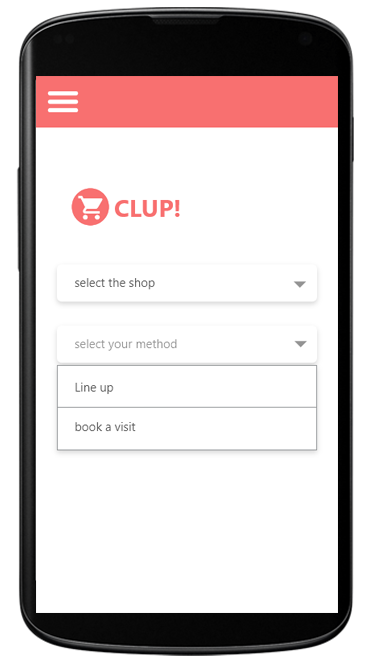
\includegraphics[width=0.4\textwidth,keepaspectratio]{images/11.png}}
  \hfill
  \caption{Mockup}
\end{figure}

Other mockups will be presented in the Design Document part for User Interfaces.
\subsubsection{Hardware Interfaces}
The software application contains three main functions and two types of actors, which require different
kinds of hardware interfaces.

• Regarding BS:
The users must own a smartphone in order to generate QR codes to access supermarkets. They
can also use a ticket machine for this purpose so that they can have the code in person.
The managers, instead, can access the system only through the App using a smartphone.They first have to register themselves to the system and then add their shops to the system. there is also a scanner which scan the validity of the tickets.

• Regarding AF1 : for booking a visit, users should have smartphone to get their QR codes otherwise they cannot use this feature.
\subsubsection{software Interfaces}
The system uses the following external interfaces:

City map
We assume that the system uses a public API to provide:
1. to the customer the possibility to see the shops location by selecting its branch name.
2. to the manager to add their shops location to the system

notification server:
This app has a system which it sends notification to customers when their turn is close 

estimation time:
The application shows an estimated time in which users can manage their time to be on the spot in time.

Communication Interfaces:
The device connects to CLup via internet connection.